\documentclass[9pt,twocolumn,twoside,lineno]{pnas-new}
% Use the lineno option to display guide line numbers if required.
% Note that the use of elements such as single-column equations
% may affect the guide line number alignment. 
\templatetype{pnasresearcharticle} % Choose template 
% {pnasresearcharticle} = Template for a two-column research article
% {pnasmathematics} = Template for a one-column mathematics article
% {pnasinvited} = Template for a PNAS invited submission

%\documentclass[12pt]{article}
%\usepackage[square,sort,comma,numbers]{natbib}
%\usepackage{times}
\usepackage[T1]{fontenc}
\usepackage[utf8]{inputenc}
%\usepackage[pdftex]{graphicx}
%\usepackage{caption}
%\captionsetup[figure]{justification=raggedright,labelfont=bf}
%\usepackage{fullpage} % 1" margins
\usepackage{tabu}
\usepackage{pdflscape}
%\usepackage{setspace}
%\setstretch{1.5}
%\usepackage{lineno}
%\usepackage{sectsty}
%\sectionfont{\nohang\centering\normalsize\sc}   % capitalize initial letters
%\subsectionfont{\nohang\centering\normalsize\rm\em}

% eat the colon so figures are labeled but have blank captions
% \makeatletter
% \renewcommand\fnum@figure[1]{\figurename~\thefigure\ignorespaces}
% \makeatother

%% Article

\title{Uplift-driven diversification in the Hengduan Mountains, a
  temperate biodiversity hotspot}

\author[a,b,1]{Yaowu Xing}
\author[a,c,1]{Richard H.\ Ree} 
% Use letters for affiliations, numbers to show equal authorship (if applicable) and to indicate the corresponding author
\affil[a]{Integrative Research Center, The Field Museum, 1400 South
  Lake Shore Drive, Chicago, Illinois 60605, USA}
\affil[b]{Xishuangbanna Tropical Botanical Garden, Chinese Academy of
  Sciences, Menglun Township, Mengla County, Yunnan 666303, China}
\affil[c]{National Institute of Ecology, 1210 Geumgang-ro,
  Maseo-myeon, Seocheon-gun, Chungcheongnam-do, South Korea}

% Please give the surname of the lead author for the running footer
\leadauthor{Xing} 

\significancestatement{Why do so many species occur in mountains? A
  popular but little-tested hypothesis is that tectonic uplift creates
  environmental conditions (new habitats, dispersal barriers, etc.)
  that increase the rate at which resident species divide and evolve
  to form new ones. In China's Hengduan Mountains region, a
  biodiversity hotspot uplifted over the last 8 million years, this
  rate does in fact show a significant increase during that time,
  relative to the rate for adjacent older mountains, and to the rate
  of species immigration. The Hengduan Mountains flora is thus made up
  disproportionately of species that evolved within the region during
  its uplift, supporting the original hypothesis and helping to
  explain the prevalence of mountains as global biodiversity
  hotspots.}

%\date{Yaowu Xing$^{1,2}$ and Richard H.\ Ree$^{1,3,*}$}

\authorcontributions{Y.X. and R.R. designed the research; Y.X. collected the
  data; Y.X. and R.R. analyzed the data; and Y.X. and R.R. wrote the paper.}

\authordeclaration{The authors declare no conflicts of interest.}

\equalauthors{\textsuperscript{1}Y.X. and R.R. contributed equally to this work.}

\correspondingauthor{\textsuperscript{2}To whom correspondence should be addressed. E-mail: rree\@fieldmuseum.org}

\keywords{ biogeography $|$ vascular plants $|$ molecular clocks $|$ dispersal $|$ speciation }

\begin{abstract}
  A common hypothesis for the rich biodiversity found in mountains is
  uplift-driven diversification---that orogeny creates conditions
  favoring rapid \textit{in situ} speciation of resident lineages. We
  tested this hypothesis in the context of the Qinghai-Tibetan Plateau
  (QTP) and adjoining mountain ranges, using the phylogenetic and
  geographic histories of multiple groups of plants to infer the tempo
  (rate) and mode (colonization vs.\ \textit{in situ} diversification)
  of biotic assembly through time and across regions. We focused on
  the Hengduan Mountains region, which in comparison to the QTP and
  Himalayas was uplifted more recently (since the late Miocene), is
  smaller in area, and richer in species. The time-calibrated
  phylogenetic analyses showed that about 8 million years ago, the
  rate of \textit{in situ} diversification increased in the Hengduan
  Mountains, significantly exceeding that in the geologically older
  QTP and Himalayas. By contrast, in the QTP and Himalayas during the
  same period, the rate of \textit{in situ} diversification remained
  relatively flat, with colonization dominating lineage
  accumulation. The Hengduan Mountains flora was thus assembled
  disproportionately by recent \textit{in situ} diversification,
  temporally congruent with independent estimates of orogeny. This is
  the first study to show quantitative evidence for uplift-driven
  diversification in this region, and more generally, to test the
  hypothesis by measuring the rate and mode of biotic assembly across
  time and space. It thus complements the more prevalent method of
  examining endemic radiations individually, and could be used as a
  template to augment such studies in other biodiversity hotspots
  (e.g., the Andes).
\end{abstract}

\dates{This manuscript was compiled on \today}
\doi{\url{www.pnas.org/cgi/doi/10.1073/pnas.XXXXXXXXXX}}

\begin{document}
% \raggedright
% \parindent 0.5in

% Optional adjustment to line up main text (after abstract) of first page with line numbers, when using both lineno and twocolumn options.
% You should only change this length when you've finalised the article contents.
\verticaladjustment{-2pt}

\maketitle

\thispagestyle{firststyle}
\ifthenelse{\boolean{shortarticle}}{\ifthenelse{\boolean{singlecolumn}}{\abscontentformatted}{\abscontent}}{}


% \noindent Author affiliations:
% \begin{enumerate}

% \item Integrative Research Center, The Field Museum, 1400 South Lake
%   Shore Drive, Chicago, Illinois 60605, USA

% \item Xishuangbanna Tropical Botanical Garden, Chinese Academy of
%   Sciences, Menglun Township, Mengla County, Yunnan 666303,
%   China %Tel: +86 691 8715071

% \item National Institute of Ecology, 1210 Geumgang-ro, Maseo-myeon,
%   Seocheon-gun, Chungcheongnam-do, South Korea

% \end{enumerate}

% \noindent * Corresponding author. Email: rree@fieldmuseum.org; +1-312-665-7857

% \bigskip

% \noindent Short title: Uplift-driven diversification in the Hengduan Mountains
% %\noindent Short title: Tempo and mode in biodiversity hotspot assembly

% \noindent Classification: Biological Sciences; Evolution


% \newpage
% \section*{Abstract}

A common hypothesis for the rich biodiversity found in mountains is
uplift-driven diversification---that orogeny creates conditions
favoring rapid \textit{in situ} speciation of resident lineages. We
tested this hypothesis in the context of the Qinghai-Tibetan Plateau
(QTP) and adjoining mountain ranges, using the phylogenetic and
geographic histories of multiple groups of plants to infer the tempo
(rate) and mode (colonization vs.\ \textit{in situ} diversification)
of biotic assembly through time and across regions. We focused on the
Hengduan Mountains region, which in comparison to the QTP and
Himalayas was uplifted more recently (since the late Miocene), is
smaller in area, and richer in species. The time-calibrated
phylogenetic analyses, which made no prior assumptions about when any
region was uplifted, showed that about 8 million years ago, the rate
of \textit{in situ} diversification increased in the Hengduan
Mountains, significantly exceeding that in the geologically older QTP
and Himalayas, and marked the point at which cumulative speciation
overtook colonization. By contrast, in the QTP and Himalayas during
the same period, the rate of \textit{in situ} diversification remained
relatively flat, with colonization dominating lineage
accumulation. This indicates that the Hengduan Mountains flora has
been assembled disproportionately by recent \textit{in situ}
diversification that coincides temporally with independent estimates
of orogeny, and is the first quantitative evidence to support the
uplift-driven diversification hypothesis.

\newpage

\section*{Significance Statement}

Why do so many species occur in mountains? A popular but little-tested
hypothesis is that mountain uplift creates environmental conditions
(new habitats, dispersal barriers, etc.) that increase the rate at
which resident species divide and evolve to form new ones. In China's
Hengduan Mountains region, a biodiversity hotspot where uplift began
about 8 million years ago, this rate does in fact show a significant
increase since that time, relative to the rate for adjacent older
mountains, and to the rate of species immigration. The Hengduan
Mountains flora is thus made up disproportionately of species that
evolved within the region during its uplift, supporting the original
hypothesis and helping to explain the prevalence of mountains in
global biodiversity hotspots.



%%% Local Variables: 
%%% mode: latex
%%% TeX-master: "master"
%%% End: 

% \newpage

\section{Introduction}

% Assembly of biodiversity hotspots - when, how, why? 2 basic processes: dispersal (immigration) and in situ diversification (speciation). Reconstructing these dynamics over time, in the context of geological and climatological events, is important to understanding the drivers/causes of major patterns in biogeography and macroecology (e.g., latitudinal diversity gradient).

Understanding when and how regional biotas were assembled is central to understanding why biodiversity is distributed unevenly on Earth. Among global biodiversity hotspots---regions of unusually high species richness and endemism---the mountains along the southern edge of the Qinghai-Tibetan Plateau (QTP) are unusual in being neither tropical nor Mediterranean in climate, and they are also enigmatic, because despite increasing interest from biogeographers, the timing, tempo, and mode of their biotic assembly remains poorly understood.

The mountains actually form 2 distinct hotspots of biodiversity, roughly demarcated by the Tsangpo River Gorge in southeastern Tibet. The richer Hengduan Mountains lie to the east, with a flora of ca.\ 12,000 species of vascular plants in ca.\ 500,000 km$^2$ (Boufford; Li, 1993 #2; Wu, 1988 #1); and the Himalayas to the west, with ca.\ 10,000 species in ca.\ 750,000 km$^2$ (REF).

Any consideration of the biogeography of these floras necessarily begins with the formation of the mountains themselves and the associated changes in climate. Uplift of the QTP is intimately associated with development of the Asian monsoon and aridification of the regions north and west of the Himalayas (reviewed by Favre et al. 2014). Generally speaking, the orogenic history of the QTP and its surrounding mountains is extremely complex, and many details are controversial, with different lines of evidence often yielding conflicting inferences (see reviews in {Wang, 2014 #216} and Deng and Ding, 2016). Nevertheless, it seems likely that the central plateau was uplifted first, reaching its current elevation as early as 51-40 Ma to as late as 28 Ma (Xu, 2013 #217; Wang, 2014 #216), with subsequent outward growth. Along the southern edge of the plateau, the Himalayas rose earlier, reaching their current elevation no later than 11-9 Ma, while the Hengduan Mountains formed later, rising mainly after 10 Ma (Wang, 2012 #218; Mulch, 2006 #81; Sun, 2011 #43).

The Hengduan Mountains are thus younger than the Himalayas and smaller in area, but richer in species. What historical biogeographic factors explain this disparity? One approach is to frame the question simply in terms of two basic processes of regional lineage accumulation: \textit{in situ} diversification and colonization. The former is commonly thought to be accelerated by mountain uplift, because topographic complexity can increase the potential for speciation via allopatric isolation of populations, and adaptive divergence along environmental/elevational gradients (REFS?). Thus we generally expect higher rates of \textit{in situ} speciation during periods of uplift. However, it is also possible that by creating and/or expanding habitats (e.g., of the alpine zone), uplift increases the potential for successful colonization by pre-adapted lineages dispersing from other regions (REFS?). Uplift, in other words, might accelerate both processes.

Compared to the Himalayas, for the Hengduan Mountains to have accumulated more species in less time means that its combined rate of \textit{in situ} diversification and colonization must have been higher over the course of its orogeny. But which process was dominant? In the literature, the hypothesis of uplift-driven diversification is clearly favored over uplift-driven colonization, being commonly invoked as an explanation for phylogenetic or phylogeographic divergences in the Hengduan Mountains (e.g., REFS). However, conspicuously lacking from these studies are quantitative analyses that explicitly measure rates of diversification and colonization, and compare them across geographic regions and time (e.g., see reviews by Wen et al and Favre et al). Consequently, the idea that uplift-driven diversification has contributed disproportionately to floristic assembly in the Hengduan Mountains has yet to be rigorously tested.

%The regions have often been considered a single floristic unit based on shared taxa (e.g., REFS).

%differ most conspicuously in their general orientation, with the Himalayas running east-west, and the Hengduan Mountains running north-south.

%Therefore, the nascent Hengduan region surely had close biogeographic connections to pre-existing alpine environments to the north and west, from which mountain-adapted clades could have dispersed. For example, in Cyananthus (Campanulaceae), phylogenetic analysis suggests that vicariance triggered by the uplift of the QTP accelerated the divergence of regional clades (sections), and that the Hengduan Mountains were colonized from the Himalayas {Zhou, 2013 #94}. More complex pattern has been found in the genus Anaphalis, (Asteraceae) that Anaphalis first radiated in the eastern Himalayas (Hengduan Mt) and migrated into eastern Asia, western Himalayas, as well as into North America, and SE Asia. This means Hengduan Mt mainly act as both species cradle and source of other floras. A general picture is still lacking and quantitative analyses are needed to address the contribution of immigration.

%None of these studies explicitly quantified diversification rates between HMH and other regions which makes hard to conclude whether extraordinary plant diversity in HMH is due to rapid diversification. Moreover, estimates of the time spans of these radiations vary widely (between 20-1.56 Ma), and in most cases are based only on secondary molecular-clock calibrations. Therefore, reconstructing the diversification rates dynamics across different clades will provide new insights into diversification processes in the HMH.

%It remains untested that how much immigration by pre-adapted species from adjacent regions had contributed to the exceptional plant diversity in the HMH. Much effort has been applied to reconstruct geographic patterns for clades in the QTP and adjacent regions (). Different hypotheses have been proposed in explaining current biogeographic pattern. Some studies indicate that most of the clades originated in the QTP and adjacent regions and started to specify in other Northern Hemisphere regions (e.g. Zhang et al., 2007, 2009; Xu et al., 2010; Zhang et al., 2014(Rhodiola)). Alternatively, some clades originated in other regions and radiated in the QTP (e.g. Liu et al., 2002; Tu et al., 2010). However, little is known when, from where and to which extent immigration has contributed to the spectacular diversity in the HMH in relative to in situ speciation. Were these biogeographic patterns associated with geological and environmental changes?

%"Uplift-driven diversification" hypothesis. Many recent phylogenetic studies of particular clades have invoked uplift of the QTP in general, and the Hengduan Mountains in particular, as a causal factor in lineage diversification. (see Favre et al 2015).

%To investigate the claim of "uplift-driven diversification", need to measure rates of in situ diversification and immigration of lineages over time. Also need to know when uplift occurred.

%If the Himalayas are indeed older than the Hengduan Mountains, we can speculate that the assembly of its flora began earlier, coinciding temporally with orogeny, and was dominated initially by a high rate of \textit{in situ} radiations of resident lineages (i.e., those already established on the southern edge of the QTP), or of early colonizing lineages from neighboring mountains, such as the Altai-Tienshan. Assuming density-dependent effects, the rate of assembly would have then tapered as the flora matured and the Himalayas approached their current height around 10 Mya. By contrast, as the Hengduan Mountains subsequently rose to the east, it seems plausible that the assembly of its flora was from the outset a more dynamic balance between colonization (primarily from the established flora of the geographically proximate and ecologically similar Himalayas) and \textit{in situ} diversification, and that the combined rates of these processes have been rising as orogeny has proceeded since the late Miocene.

In this study we develop a phylogenetic framework for inferring region-specific rates of diversification and colonization through time that combines fossil-calibrated molecular clocks for divergence-time estimation, historical biogeographic inferences of ancestral ranges and movements, and reconstructions of macroevolutionary birth-death regimes. We use it to infer the dynamics of floristic assembly in the Hengduan Mountains and Himalayas, with the primary aim of discovering the historical differences in assembly processes that explain the richer Hengduan flora.

%Methods of inferring biogeographic dynamics over evolutionary timescales. Fossil record - track the diversity and occurrence of species/clades in space directly through time. Alternatively, use time-calibrated phylogenies of extant species, and inferences of historical biogeography - where were lineages in the past, where did they diversify, and when/how did they move between regions. Both approaches: issue of sampling - incompleteness, bias. Phylogenies/anc. range reconstruction: issue of extinction.

%In this study we study the historical assembly of the Hengduan Mountains biodiversity hotspot using biogeographic inferences from multiple clades of seed plants. Our primary goal is to test the hypothesis that, compared to the Himalayas, its richer flora is the result of higher rates of \textit{in situ} diversification than immigration. A secondary hypothesis is that lineage-range dynamics in the Hengduan Mountains over time are qualitatively distinct from those in adjacent regions - that is, we wish to study the empirical justification for distinguishing it from the Himalayas. Multiple clades: time-calibrated phylogenies, species ranges. Ancestral range reconstruction yields inferences about when and how lineages moved and proliferated, integrated over uncertainty in topologies, node ages, and precise sequences of events.
\section*{Results}

\subsection*{Contrasting histories of floristic assembly}

Reconstructed biogeographic histories of the selected clades reveal distinct patterns of floristic assembly across regions when plotted as the cumulative number of colonization and \textit{in situ} speciation events through time (Fig.~\ref{fig:cumevents}). Given geological and paleontological evidence that the Hengduan Mountains are younger than the Himalayas-QTP, we expected to find that its flora was assembled more recently. Instead, we found surprisingly deep phylogenetic histories of Hengduan occupancy, with initial assembly of its flora pre-dating that of the Himalayas-QTP. In more than 95\% of the pseudoreplicated joint histories, the earliest colonization event occurs by 88 Ma for the Hengduan Mountains and by 56 Ma for the Himalayas; \textit{in situ} speciation begins later, starting by 35 Ma and 20 Ma, respectively. By contrast, in East Asia, which was commonly reconstructed as the root ancestral area for clades, \textit{in situ} speciation initially occurs by 106 Ma and colonization initially occurs by 78 Ma.

For all regions, species accumulation by each process is approximately exponential (log-linear) following initiation until about the last 8 Ma. During this earlier "constant" phase, assembly in both the Hengduan Mountains and Himalayas-QTP is dominated by colonization, while in temperate/boreal East Asia the dominant process is \textit{in situ} speciation. Following this phase, the assembly dynamics of the Hengduan Mountains and Himalayas diverge considerably, with relatively little change in temperate/boreal East Asia. In the Hengduan Mountains, the cumulative number of \textit{in situ} speciation events overtakes that of colonization around 8 Ma, and by the present, the median number is 496 versus 345. In the Himalayas-QTP, \textit{in situ} speciation never overtakes colonization, and by the present the median number of events is 192 versus 416. The relative contribution of \textit{in situ} speciation to floristic assembly is thus $496/(496+345) = 0.590$ for the Hengduan Mountains, and $192/(192+416) = 0.316$ for the Himalayas-QTP. In other words, \textit{in situ} speciation has contributed about twice as much to the assembly of the Hengduan Mountains flora as it has to the Himalayas-QTP flora, especially since the late Miocene.

\subsection*{Regional rates of \textit{in situ} speciation and dispersal through time}

The rate of \textit{in situ} speciation for the Hengduan Mountains region, in events per resident lineage per Ma, increased almost twofold over the past 10 Ma, while for the Himalayas-QTP, it remained more or less constant (Fig.~\ref{fig:speciation}). Dispersal rates between the Hengduan Mountains and Himalayas-QTP increase gradually over the last 4--5 Ma, and sharply in the last 1 Ma. By contrast, dispersal from each region to temperate/boreal East Asia increases only slightly in the same time period (Fig.~\ref{fig:dispersal}).

\subsection*{Shifts in diversification rate}

Seven out of the 18 clades showed strong evidence (Bayes factor > 15) for one or more shifts in diversification regime (Table~\ref{table:bammbayesfactors}). However, inspection of branch-specific evidence (the cumulative probability of occurring in the credible set of shift configurations, and the marginal odds ratio in favor of a shift) in light of ancestral-range reconstructions does not reveal any clear geographic patterns in the phylogenetic locations of regime shifts (Fig.~S2). That is, across clades, macroevolutionary jumps in diversification rate are not obviously associated with the colonization or occupancy of any particular region.

A notable exception to this general pattern is \emph{Rhododendron}, in which results from BAMM and Lagrange suggest that in a window of about 9--15 Ma, net diversification increased independently in 2 clades that each originated in the Hengduan region and are currently dominated by Hengduan species (Fig.~\ref{fig:rhododendron}). In \emph{Saussurea}, an increase in net diversification is inferred about 1.7 Ma along the stem of a branch containing most of the clade's Hengduan species (Fig.~S??). Similarly, in Delphineae, 2 separate increases are inferred in clades that are ancestrally Hengduan and together hold most of the Hengduan species; however the times of these rate shifts (about 28 Ma and 37 Ma, respectively) pre-date the uplift of the Hengduan Mountains (Fig.~S??). Finally, in \emph{Isodon} and \emph{Ligularia}, branch-specific measures show one increase in net diversification for each clade in the context of Hengduan ancestry about 7 and 5 Ma, respectively, but in both cases, models with regime shifts are not supported by Bayes factors, and the Hengduan Mountains region is reconstructed as ancestral across most of the phylogeny, rendering the geographic context of the shift less informative.

%%% Local Variables:
%%% mode: latex
%%% TeX-master: "master"
%%% End:

\section{Discussion}

Our analysis is the first to make quantitative temporal inferences about the relative contributions of \textit{in situ} lineage diversification and colonization to the assembly of one of the world's richest temperate floras. Despite precedent in the literature for considering the Hengduan Mountains to be simply part of a greater biogeographic region that includes the Himalayas and QTP \citep[e.g.][]{Zhang2014,Nie2013,GaoY2013,Matuszak2016}, we instead find that the Hengduan region actually has a very distinct history of assembly that reflects its younger age.

We expected regional differences to reflect contrasting times of orogeny: in particular, the uplift-driven diversification hypothesis predicts that \textit{in situ} speciation increases with mountain-building activity. In this context the late Miocene (12--8 Ma) is an important reference point, as previous studies of geology and paleontology indicate that the Hengduan Mountains achieved their current height only after this time, while the Himalayas and central QTP did so before (REFS). Here, our phylogenetic inferences, which make no prior assumptions about the timing of geological events, show that after about 8 Ma, the rate of \textit{in situ} speciation increased in the Hengduan Mountains, yielding a remarkable inflection point at which cumulative speciation overtakes colonization. This indicates that the Hengduan Mountains flora has been assembled disproportionately by recent \textit{in situ} speciation that coincides temporally with independent estimates of orogeny, supporting (at least superficially) the uplift-driven diversification hypothesis.

We do not find a similar signature of accelerated \textit{in situ} speciation for the Himalayas-QTP region, as might be expected from rapid Himalayan orogeny during the early to middle Miocene (REFS: Searle 2011?)  % \citep{WangY2007,Mao2010}
. It is possible that no such pulse of diversification occurred, e.g., if uplift of the Himalayas was more gradual. Alternatively, we could simply lack the statistical power to detect it, due to the masking effects of lumping the older QTP with the younger Himalayas, the greater uncertainty associated with estimating clade ages and ancestral ranges in deeper time, and/or extinction and turnover in the Himalayas-QTP flora.

% From Fig.2, speciation rate of Himalayas also increased until around 8 Ma, and keep constant since then. This probably due to Himalayas already reached its current elevation.

The older age of the Himalayas-QTP predicts that its flora should have been an early source of lineage dispersal to the younger Hengduan Mountains, which acted as a colonization sink. However, we do not find any marked asymmetry in dispersal between these regions through the end of the Miocene; instead, rates in both directions are relatively low and increase only gradually until about 2--3 Ma, when both increase more sharply, but more so from the Hengduan Mountains to the Himalayas-QTP (Fig.~\ref{fig:dispersal}). That is, in the Quaternary, the Hengduan Mountains appear to have acted more as a biogeographic \textit{source} than a sink for the Himalayas-QTP. This may reflect phylogeographic evidence that the Hengduan Mountains flora was likely buffered from extinction during Quaternary glacial cycles, with subsequent westward range expansion/recolonization of the Himalayas and QTP \citep[e.g.,][]{WangBS2011,CunY2010}. 

%Surpringly, our results indicate Himalayas-QTP flora was assembled later (Fig **). Ideally, bring paleontological evidence to bear on assembly/diversification questions - but the record is sparse. The exact time of onset of current biome remains unclear.

\textbf{Lack of correspondence between dispersal and shifts in diversification.}---Given the result that \textit{in situ} speciation is the dominant process in the Hengduan Mountains since the late Miocene, the lack of evidence for macroevolutionary jumps in diversification rate associated with colonization of the region might seem surprising. However, across our phylogenies, dispersal is relatively frequent and clades tend not to be entirely endemic to a single region. This reflects the fact that our regions are not, in general, defined by differences in biome; the Hengduan Mountains, Himalayas, and QTP share broad physiographic similarities that presumably have facilitated biogeographic exchange. That is, dispersal between regions should not necessarily require extensive ecophysiological adaptations that may be difficult to evolve \citep{Donoghue2014}, tempering expectations of evolutionary radiations within a region \citep[cf.][]{Hughes2006}. For this reason our data are perhaps not well-suited for BAMM, which models diversification shifts as relatively rare events. Moreover, the link between dispersal events and shifts in diversification regime is further obscured by the inherent uncertainty associated with inferring their phylogenetic locations.

The most appropriate interpretation may simply be that the signal of higher diversification in the Hengduan region is more or less diffuse across clades, and emerges only when their biogeographic histories are considered jointly. This helps explain why previous analyses of single clades have not yielded the pattern inferred here.

\textbf{Drivers of Hengduan diversification.}---How and why did \textit{in situ} diversification in the Hengduan Mountains increase since the late Miocene, and more specifically, to what extent was it driven by orogeny? Further studies are needed. One might look for contrasts between the Hengduan Mountains and adjacent regions in the evolution of ecological traits and environmental tolerances \citep[e.g.,][]{liu2016} across multiple clades. These may reveal, for example, the extent to which speciation within a region is associated with adaptive divergence and niche-filling \citep{price2014}, as opposed to nonadaptive processes such as genetic isolation and drift arising from topographic effects (vicariance, emergence of sky islands, etc.). These analyses would require denser and more fine-grained taxonomic and geographic sampling than was possible here, in addition to the requisite trait data.

% Aridification and global cooling as a result of orogeny (see reviews in \citealt{MiaoY2012}) may be an important factor influencing the diversification of plants on the QTP.

We suspect that evidence for common processes will prove elusive, as the proximate causes of diversification are likely to be idiosyncratic. For many clades, factors unrelated to uplift \emph{per se}, such as biotic interactions, are almost certain to have played important roles. For example, in \emph{Pedicularis} (Orobanchaceae), diversification of the many Hengduan species may have been facilitated by recurrent divergence in floral traits associated with pollinator sharing and reproductive interference \citep[e.g.,][]{eaton2012}.

A coarser-grained view is that diversification in the Hengduan region reflects a macroevolutionary response to greater niche availability, primarily driven by the rapid expansion of moist temperate montane and alpine habitats in the late Miocene. At this level the effects of orogeny and climate change are not clearly separable, but jointly set a stage of ecological/evolutionary opportunity. During the early to middle Miocene, the southern QTP had already achieved its current elevation \citep{Spicer2003} and was covered by coniferous and deciduous-leaved forests \citep{SunJ2014,LiH1976}% , and limited paleobotanical evidence suggests that the entire Himalayas-QTP region may have experienced a dramatic shift in vegetation after the middle Miocene
. As Hengduan uplift proceeded, falling temperatures would have driven the treeline lower, increasing the extent of shrublands, meadows, and scree slopes---habitats where most of the species in our data set occur and would have diversified. Similar changes would also have occurred in the Himalayas and QTP, but in comparison to those areas, moisture in the Hengduan region would have been abundant, as by then, the summer monsoon was established, and the central QTP and Central Asian interior had aridified \citep[see][]{Renner2016}. This predicts that carrying capacities---and by extension, diversification potential---of the Hengduan region's newly formed habitats were enhanced by greater summer rainfall. 

% Accounting for the effect of Pleistocene climate fluctuations

While not a driver of diversification \textit{per se}, it is important to consider the effects of glaciation and climatic oscillations during the Pleistocene, and the possibility that our results can be explained, at least in part, by regional differences in extinction caused by these factors. If the Hengduan region had more Pleistocene refugia, we would expect its history of \textit{in situ} diversification to be better preserved in time-calibrated phylogenies, simply because fewer branches would have been ``pruned'' by extinction. By contrast, greater extinction in the Himalayas-QTP, if phylogenetically random, would tend to erase nodes representing recent \textit{in situ} speciation events, and increase the average nearest-phylogenetic-neighbor distance for pre-Pleistocene resident survivors. That is, even if regional rates of \textit{in situ} diversification were equal up to the Pleistocene, we might infer the rate to be higher in the region that experienced less Pleistocene extinction.

Numerous studies of species distributions \citep[e.g.,][]{srinivasan2014,lopez2011} and phylogeography \citep[e.g.,][]{CunY2010,WangBS2011,lei2014,meng2015} support the idea that refugia were concentrated along the southeastern margin of the QTP, but also occurred in areas further west and north, even at high elevation \citep[e.g.,][]{wang2009,sun2010,opgenoorth2010}. This is in line with geological evidence that ice-free areas were present across the QTP and adjacent mountains throughout the Quaternary \citep[see][]{owen2014}. It may be that greater Pleistocene extinction in the Himalayas-QTP compared to the Hengduan region was driven as much (or more) by aridification as glaciation, during periods of reduced summer monsoon strength associated with local interglacials \citep{owen2008}.

% even paleoelevational recontruction suggesting this regions already reached their current elevation by then . The onset and diversification of alpine biome may be much later than the uplift.

% More generally, it seems reasonable to view uplift and climate change as primary drivers of expanding ecological opportunities for temperate-montane species in the Hengduan region in the late Miocene.

\textbf{Comparisons to other taxa, mountains, and hotspots.}---Our results in plants qualitatively resemble similar patterns found in numerous single-clade studies of 

% In this study we attempt to place the Hengduan Mountains flora in historical biogeographic context through the joint analysis of representative clades. The picture that emerges is one in which \textit{in situ} diversification accelerates relative to colonization around the time orogeny is believed to have started.

In the Introduction, we considered the processes of \textit{in situ} diversification and colonization as equally likely a priori to contribute to the assembly of biodiversity hotspots. We find that diversification wins. The question then becomes: is this a general result, or specific to the unique circumstances of the Hengduan Mountains, and therefore unpredictable?

Most similar to Cerrado \citep{simon2009}. In that study, the focus was on a particular biome, and the evolution of traits required to thrive in that biome.

What do our results illustrate about the assembly of biodiversity in the Hengduan Mountains in particular, or biodiversity hotspots/mountains in general



% \textit{In situ} diversification also implicated in the assembly of other biodiversity hotspots: the Andes, California Floristic Province (Kay and Lancaster?), Cape Floristic Region? Uplift-driven diversification: Andes, Japan?
How is the Hengduan Mountains region similar to other biodiversity hotspots? How does it differ? The Hengduan Mountains region is a young biodiversity hotspot. Young hotspots contradict the general expectation that diversity is a function of time (Fine and Ree).

Comparison to paramo study: net diversification only, no dispersal; how did they define ``paramo'' clades (and clades of other hotspots)?

Comparison with northern Andes: both are young mountain regions. May reveal general properties of uplift-driven diversification.

% General considerations: ecological opportunities. Age, area, and environmental factors (moisture, temperature, seasonality, soil characteristics) influencing energy-diversity expectations.

% Age: Hengduan Mountains are young; within it, alpine biome even younger

%  extant diversity, and historical diversification (to the extent it can be inferred), reflects regional carrying capacities through time. 

% An important consideration in this context is climatic conditions over time---moisture and temperature in particular---that influence primary productivity,  

% Density-dependent effects: Himalayas are older, are niches more filled relative to Hengduan Mountains?

% Pleistocene effects: differential extinction. Young clades: Saussurea

% Perenniality, woodiness are something like ``classic'' traits associated with alpine radiation (Hughes and Atchison) - but our clades include many herbaceous species. Hybridization (Rhododendron: Milne). Sky islands (e.g., Solms-Laubachia): does population isolation lead to the proliferation of narrow endemics (that are more prone to extinction)?

% Younger clades like Saussurea - ecological opportunity of new alpine habitat?

% Predict that earliest clades are montane, most recent radiations are alpine. Not entirely the case. Pinaceae, Acer, Delphineae are montane, and colonize early. Alpine clades like Saussurea and Ligularia colonized later and with exeptional high rates (Saussurea has crown age c. 3 Myr, but has generated more than 400 species). But Meconopsis(true???), Saxifragaceae, and Polygoneae have many alpine members (Saxifragaceae and Polygoneae include many montane even low land species as well), and are the earliest clades to accumulate \textit{in situ} speciation events in the Hengduan Mountains.

% Notably, clades that occur primarily in the relatively arid alpine zone, such as \textit{Saussurea} and \textit{Rhodiola}, show faster diversification in the past 10 Ma than montane clades such as Primulaceae (s.s.) and \textit{Cyananthus}. However, precipitation is not a limiting factor in north-south-going Hengduan Mountains since moist air from the Indian Ocean can go through by the valleys, facilitating diversification of montane clades like \textit{Rhododendron} and Primulaceae (s.s.). 

% Early uplift of the plateau: what was the biome of the proto-QTP during the Eocene, Oligocene---presumably forests? Lagrange reconstructions of Hengduan (and Himalayan) ancestry that pre-date the origins of these mountains may indicate high-elevation ancestors

% how old is the alpine biome in HM, Him? Prediction: alpine flora: young species, recent colonists

% Uplift-driven diversification is either a too-simplistic hypothesis that fails to acknowledge the numerous other factors that likely contribute to biological diversification in mountains, or a too-vague catchall phrase that encompasses them all.

% Here we have found temporal alignment of elevated diversification and orogeny, with evidence coming from the joint analysis of many clades, which suggests that uplift may have had a general effect.

Rapid evolutionary radiations of plants have been documented in most major mountain ranges worldwide \citep[reviewed in][]{Hughes2015}, including the European Alps \citep{Roquet2013}, Andes \citep[e.g.][]{Hughes2006,Luebert2014}), Rocky Mountains \citep{DrummondC2012}, New Zealand \citep{Joly2014}, and the East African Rift mountains \citep{Linder2014}. Most of these have been dated to the last 5 Ma, conciding with or occurring much later than orogeny. Apparently, the Hengduan mountain radiation is older dating back to 8--10 Ma. Andes is comparable with the Himalayas-QTP and the Hengduan mountains in several ways. They habor the most alpine diversity among the mountain ranges. The initial uplift of Andes and QTP dated back to late Eocene \citep{Gregory-Wodzicki2000,Graham2009}, but plant radiations are more influenced by recent uplift (late Miocene and onwards) \citep{Hughes2013,Luebert2014,Hughes2015,Madrinan2013}. \citet{Hughes2013} pointed out that different biomes in the Neotropics may have different evolutionary histories. It is probably the case in the Himalayas-Hengduan Mountains as well. 

OTHER TAXA: BIRDS: parrotbills \citep{liu2016}

\textit{in situ} divergence and speciation along elevational gradients not important; assembly of Himalayan avifauna by colonization \citep{johansson2007}

HIGHLIGHT NEED TO STOP LUMPING WITH ``HIMALAYAS''

\textbf{Sources of error and bias.}---Taxon sampling: incomplete, and in some cases not geographically representative (Saxifragaceae). However, our focus is on relative dynamics: comparing \textit{in situ} speciation to colonization (not absolute rates of either process) and comparing the Hengduan Mountains to the Himalayas, and both to the rest of temperate East Asia. So we generally expect the results to be unbiased with respect to our hypotheses.

Granularity. To place the biogeographic assembly of the Hengduan Mountains and adjacent regions in a global context, it was necessary to adjust the granularity of the geographic coding of species. In particlar, we lumped the Himalayas with the rest of the Qinghai-Tibetan Plateau, creating a composite region of heterogeneous ages.


%%% Local Variables:
%%% mode: latex
%%% TeX-master: "master"
%%% End:

%\section{Materials and Methods}

\subsection{Clade selection and phylogeny reconstruction}

Our criteria were that each clade (1) included a substantial number of species that occur in the Hengduan Mountains, as well as their closest known relatives in other biogeographic regions; (2) had sufficient molecular data available to infer a phylogeny that was broadly representative of the clade's taxonomic diversity and geographic range; and (3) had fossil data suitable for molecular clock calibration or secondary calibrations inferred from fossil dated phylogenies. We found 18 clades---16 of angiosperms and one each of gymnosperms (Pinaceae) and ferns (Microsorioideae)---that met these criteria. The combined taxon sample included a total of 3,262 ingroup species, of which 899 occur in the Hengduan Mountains region, 624 in the Himalayas-QTP, and 1,165 in the remainder of temperate/boreal East Asia (see \textit{Delimitation of biogeographic regions}). Of these, about 370 species are shared by the Hengduan Mountains and Himalayas-QTP regions. Across clades, the proportion of species sampled ranged from 20--97\% globally and 40--97\% for the Hengduan Mountains region (Table S1).

For each clade, we assembled molecular sequence alignments (Table S2; \textit{Appendix 1}) and fossil calibration data, and used relaxed molecular clock models implemented in BEAST 1.8 \citep{Drummond2012} or 2.0 \citep{Bouckaert2014} to generate a Bayesian posterior sample of time-calibrated phylogenies and the associated maximum-clade-credibility tree.  Detailed information is provided in \textit{SI Materials and Methods}.

%, representing approximately XX\%, YY\%, and ZZ\% of the vascular flora of each region (SI REF).

\subsection{Inference of range evolution and lineage diversification}

\subsubsection{Delimitation of biogeographic regions}

We defined 11 biogeographic regions (Fig.~S1), balancing considerations of model complexity, the need to accommodate the global distributions of the selected clades, and the granularity of our species range data. Of primary importance was distinguishing the Hengduan Mountains region from the geologically older parts of the QTP, especially the Himalayas. To that end, our definition of the Hengduan Mountains region follows \citet{Boufford2014}, and is bounded to the west by the Yarlung Tsangpo River in eastern Xizang (Tibet), to the northwest by the high plateau in Qinghai, to the north by the Tao River in southern Gansu, to the east by the Sichuan Basin, and to the south by subtropical forests and the Yunnan–Guizhou Plateau. As a primary point of comparison, we defined the ``Himalayas-QTP'' region as including the plateau itself, the Himalayas to the south, the Kunlun Mountains to the north, and the Qilian Mountains to the northeast. The other regions we defined are: temperate/boreal East Asia (the eastern boreal part of Russia and temperate regions of East Asia, including Japan and Taiwan); central/western Asia (including the Xinjiang Uyghur Autonomous Region to the south of Kunlun Range); southeast Asia (including tropical regions of China, Malesia, and Papuasia); Australasia (Australia, New Zealand, and the southwestern Pacific); India (south of the Himalyas, including Sri Lanka); Africa; Europe; North America; and South America (south of the Panama Canal). We scored the geographic range of each sampled species as its presence or absence in these regions based on floras, online databases, and published data sets (\textit{Dataset S1}; see also \textit{SI Materials and Methods}).

\subsubsection{Ancestral range reconstruction}

We set up a DEC model of range evolution in Lagrange \citep{Ree2005,Ree2008}, specifying a region-adjacency matrix that defined the valid set of spatially contiguous ranges. We explicitly avoided placing any temporal constraints on dispersal, so that biogeographic inferences were independent of prior beliefs about the ages of the Hengduan Mountains or Himalayas-QTP regions. For each clade, we used the model to infer a distribution of phylogenetic histories of biogeographic events. A single history for a clade was generated by sampling a chronogram from its Bayesian posterior distribution, estimating the maximum-likelihood set of ancestral ranges (geographic speciation scenarios) at internal nodes, and randomly interpolating parsimonious sequences of dispersal and local extinction events along branches having different ancestral and descendant ranges. This yielded a complete chronology of biogeographic events, i.e., where and when ancestral lineages moved and underwent speciation and local extinction. To account for phylogenetic uncertainty, one history was generated for each of 500 chronograms drawn randomly from the posterior for each clade. For further details, see \textit{SI Materials and Methods}.

\subsubsection{Regional assembly processes through time}

We focused our analysis on the dynamics of the Hengduan Mountains region in comparison to the Himalayas-QTP and temperate East Asia. Our objective was to estimate, for each region, rates of \textit{in situ} diversification and colonization and their cumulative contributions to biotic assembly through time. Taking the biogeographic histories of clades from the ancestral-range analysis, we generated 500 pseudoreplicated joint histories---sets of one history drawn randomly from each clade's pool without replacement. From each joint history, we extracted the chronology of \textit{in situ} speciation, colonization, and local extinction events affecting the 3 regions of interest and binned them into 1 Myr periods. This allowed region-specific estimates of assembly processes through time. We calculated rolling estimates of \textit{in situ} speciation rates as $\lambda(t) = s(t)/n(t-1)$, where $s(t)$ is the number of \textit{in situ} speciation events inferred in a region in a 1-Myr period $t$ and $n(t-1)$ is the number of inferred lineages in the region in the previous period (the cumulative sum of \textit{in situ} speciation and colonization minus local extinction). We also calculated rolling rates of colonization between regions as $d_{ij}(t) = c_{ij}(t)/n_i(t-1)$, where $c_{ij}(t)$ is the number of inferred colonization events of area $j$ from area $i$. For all estimates, confidence intervals (5--95\% quantiles) were calculated from the pseudoreplicated joint histories. Further details are provided in the \textit{SI Materials and Methods}.

\subsubsection{Geography-independent rates of diversification}

To complement the regional-process analysis and to better understand heterogeneity in rates of lineage diversification independently of geography, we generated Bayesian inferences of diversification rate for each clade using BAMM \cite{Rabosky2014}, which uses Markov chain Monte Carlo procedures to jointly estimate the number, parameters, and locations of distinct macroevolutionary regimes (rates of lineage birth and death, possibly time-dependent) on a phylogenetic tree. BAMM is able to account statistically for incomplete taxon sampling, so we assigned sampling fractions at the finest level of taxonomic resolution possible: this was generally at the level of genus, but at the level of section for \textit{Rhododendron} and \textit{Acer}. In cases where genera were not confidently resolved as monophyletic, we assigned sampling fractions at the higher taxonomic levels (tribe and subfamily). We ran each BAMM MCMC for 100 million generations with a sampling frequency of 1000 and assessed convergence by visually inspecting plots of the likelihood trace and calculating the effective sample size after discarding the first 10\% of the run as burn-in. We identified the 95\% credible set of distinct shift configurations and the overall best set of rate shifts given the data using the BAMMtools package in R \cite{Rabosky2014}.



\clearpage

\begin{landscape}

\begin{table}[th]
  \caption{Bayes factor support for shifts in diversification in sampled clades, relative to the null hypothesis of no shifts. Strong support (value $>$ 15) is indicated in bold.}
  \begin{tabu} to \linewidth {X[-2,l,b]X[-1,r,b]X[-1,r,b]X[-1,r,b]X[-1,r,b]X[-1,r,b]X[-1,r,b]X[-1,r,b]X[-1,r,b]X[-1,r,b]X[-1,r,b]X[-1,r,b]}
    \hline
    & \multicolumn{11}{c}{number of regime shifts} \\
    Clade                               & 1               & 2                & 3                & 4                & 5                & 6                & 7                & 8                & 9                & 10              & 11     \\
    \hline
    \textbf{\textit{Acer}}              & \textbf{31.76}  & \textbf{71.62}   & \textbf{26.07}   & 5.59             & 1.05             & 0.12             &                  &                  &                  &                 &        \\
    \textbf{\textit{Allium}}            & 14.24           & \textbf{182.48}  & \textbf{1048.16} & \textbf{3836.48} & \textbf{6668.16} & \textbf{7038.72} & \textbf{5401.60} & \textbf{3015.68} & \textbf{1382.40} & \textbf{409.60} & 163.84 \\
    Clematidinae+Anemoninae             & 6.74            & 6.82             & 4.10             & 1.72             & 0.44             & 0.16             & 0.05             &                  &                  &                 &        \\
    \textit{Cyananthus}                 & 0.96            & 0.52             & 0.18             & 0.06             & 0.02             & 0.00             &                  &                  &                  &                 &        \\
    \textbf{Delphineae}                 & \textbf{377.43} & \textbf{5871.71} & \textbf{6889.71} & \textbf{4316.57} & \textbf{1872.00} & \textbf{566.86}  & \textbf{137.14}  & \textbf{36.57}   &                  &                 &        \\
    \textit{Isodon}                     & 8.18            & 8.60             & 5.23             & 2.23             & 0.94             & 0.19             & 0.06             &                  &                  &                 &        \\
    \textit{Ligularia-Cremanthodium-Parasenecio} complex                  & 1.64            & 1.41             & 0.80             & 0.32             & 0.12             & 0.04             & 0.01             &                  &                  &                 &        \\
    \textit{Lilium}+\textit{Nomocharis} & 0.17            & 0.041            & 0.01             &                  &                  &                  &                  &                  &                  &                 &        \\
    \textit{Meconopsis}                 & 0.77            & 0.32             & 0.10             & 0.02             & 0.01             &                  &                  &                  &                  &                 &        \\
    Microsoroideae                      & 3.83            & 4.37             & 2.79             & 1.19             & 0.38             & 0.11             & 0.07             &                  &                  &                 &        \\
    \textbf{Pinaceae}                   & \textbf{40.78}  & \textbf{29.36}   & 10.15            & 2.17             & 0.34             & 0.05             &                  &                  &                  &                 &        \\
    \textbf{Polygoneae}                 & \textbf{550.12} & \textbf{1841.18} & \textbf{7241.41} & \textbf{8086.59} & \textbf{5225.41} & \textbf{2304.00} & \textbf{783.06}  & \textbf{165.65}  &                  &                 &        \\
    Primulaceae                         & 2.13            & 2.18             & 1.54             & 0.77             & 0.36             & 0.09             & 0.06             & 0.02             &                  &                 &        \\
    \textit{Rhodiola}                   & 1.94            & 1.92             & 1.33             & 0.71             & 0.26             & 0.08             & 0.02             &                  &                  &                 &        \\
    \textbf{\textit{Rhododendron}}      & \textbf{17.76}  & \textbf{87.97}   & \textbf{247.00}  & \textbf{289.51}  & \textbf{215.75}  & \textbf{111.64}  & \textbf{40.47}   & 9.76             & 2.30             &                 &        \\
    \textit{Rosa}                       & 1.31            & 0.90             & 0.42             & 0.18             & 0.03             & 0.01             &                  &                  &                  &                 &        \\
    \textbf{\textit{Saussurea}}         & 7.30            & \textbf{20.21}   & \textbf{21.68}   & 13.56            & 6.26             & 2.01             & 0.35             &                  &                  &                 &        \\
    Saxifragaceae+Grossulariaceae       & 1.91            & 1.52             & 0.72             & 0.26             & 0.04             & 0.00             &                  &                  &                  &                 &        \\
    \textit{Thalictrum}                 & 1.57            & 1.25             & 0.67             & 0.28             & 0.10             & 0.02             & 0.01             &                  &                  &                 &        \\
    \hline
    
  \end{tabu}
  \label{table:bammbayesfactors}
\end{table}

\end{landscape}

%%% Local Variables: 
%%% mode: latex
%%% TeX-master: "master"
%%% End: 


\begin{figure}
\centering
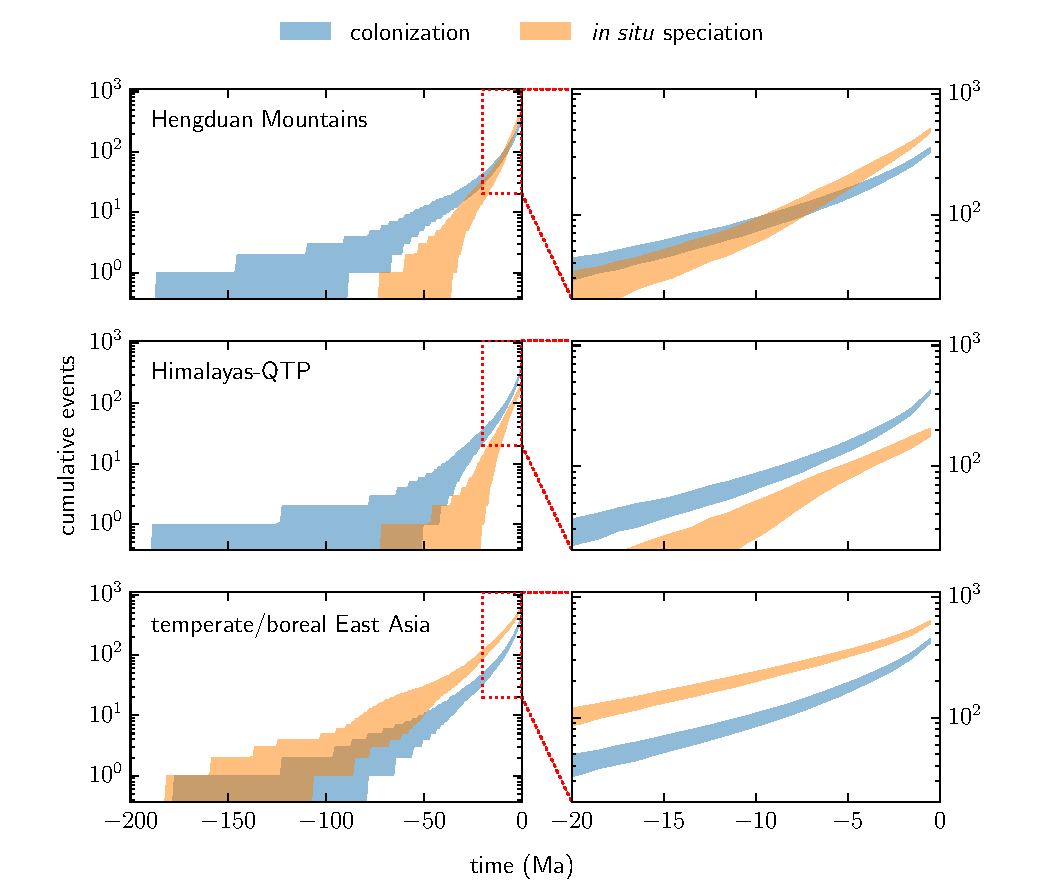
\includegraphics[width=.99\linewidth]{figures/figure_cumulative_events/figure_cumulative_events.pdf}
\caption{Assembly of regional floras by colonization and \textit{in
    situ} speciation events in 19 plant clades, inferred from
  ancestral-range reconstructions on time-calibrated molecular
  phylogenies. Shaded regions indicate the 5--95\% quantile intervals
  for the cumulative number of events through time from 500
  pseudoreplicated joint biogeographic histories designed to account
  for phylogenetic uncertainty (see text). Panels on the right focus
  on the last 20 Ma, in which differences in regional assembly are
  most apparent. In the Hengduan Mountains region, cumulative
  \textit{in situ} speciation overtakes colonization about 8 Ma,
  whereas for the Himalayas-QTP, colonization remains the dominant
  process. \textit{In situ} speciation thus appears to have played a
  disproportionately large role in assembling the Hengduan Mountains
  flora since the late Miocene compared to the Himalayas-QTP,
  consistent with the theory of uplift-driven diversification in the
  Hengduan Mountains region.}
\label{fig:cumevents}
\end{figure}

\begin{figure}
\centering
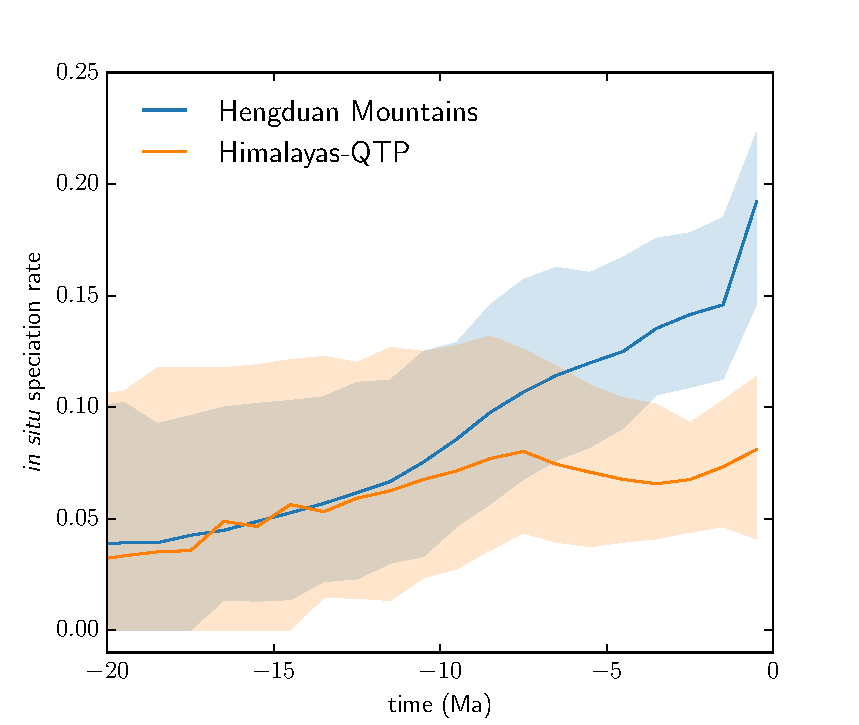
\includegraphics[width=.99\linewidth]{figures/figure_speciation_rates/figure_speciation_rates.pdf}
\caption{Rolling estimates of \textit{in situ} speciation rates
  through time for the Hengduan Mountains and Himalayas-QTP regions
  from inferred biogeographic histories of 19 plant clades. Lines
  indicate medians and shaded areas indicate 5--95\% quantile
  intervals from 500 pseudoreplicated joint histories designed to
  account for phylogenetic uncertainty (see text). Regional rates
  begin to diverge about 8 Ma, with the Hengduan Mountains showing a
  striking increase in \textit{in situ} speciation relative to the
  Himalayas-QTP.}
\label{fig:speciation}
\end{figure}

\begin{figure}
\centering
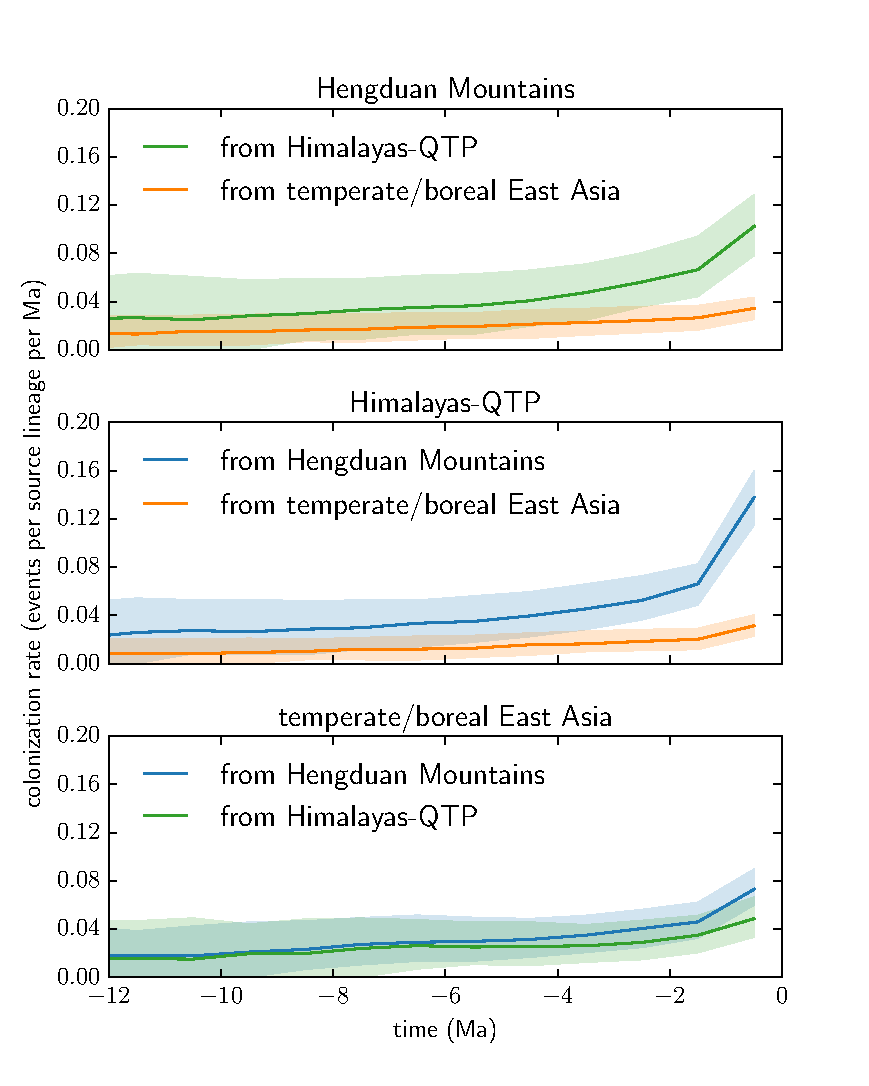
\includegraphics[width=.99\linewidth]{figures/figure_dispersal_rates/figure_dispersal_rates.pdf}
\caption{Rolling estimates of colonization rates through time for the
  Hengduan Mountains, Himalayas-QTP, and temperate/boreal East Asia
  regions from inferred biogeographic histories of 19 plant
  clades. Lines indicate medians and shaded areas indicate 5–95\%
  quantile intervals from 500 pseudoreplicated joint histories
  designed to account for phylogenetic uncertainty (see
  text). Dispersal between the Hengduan Mountains and Himalayas-QTP
  increases in the last 2 Ma relative to dispersal between either
  region and temperate/boreal East Asia.}
\label{fig:dispersal}
\end{figure}

\begin{figure}
\centering
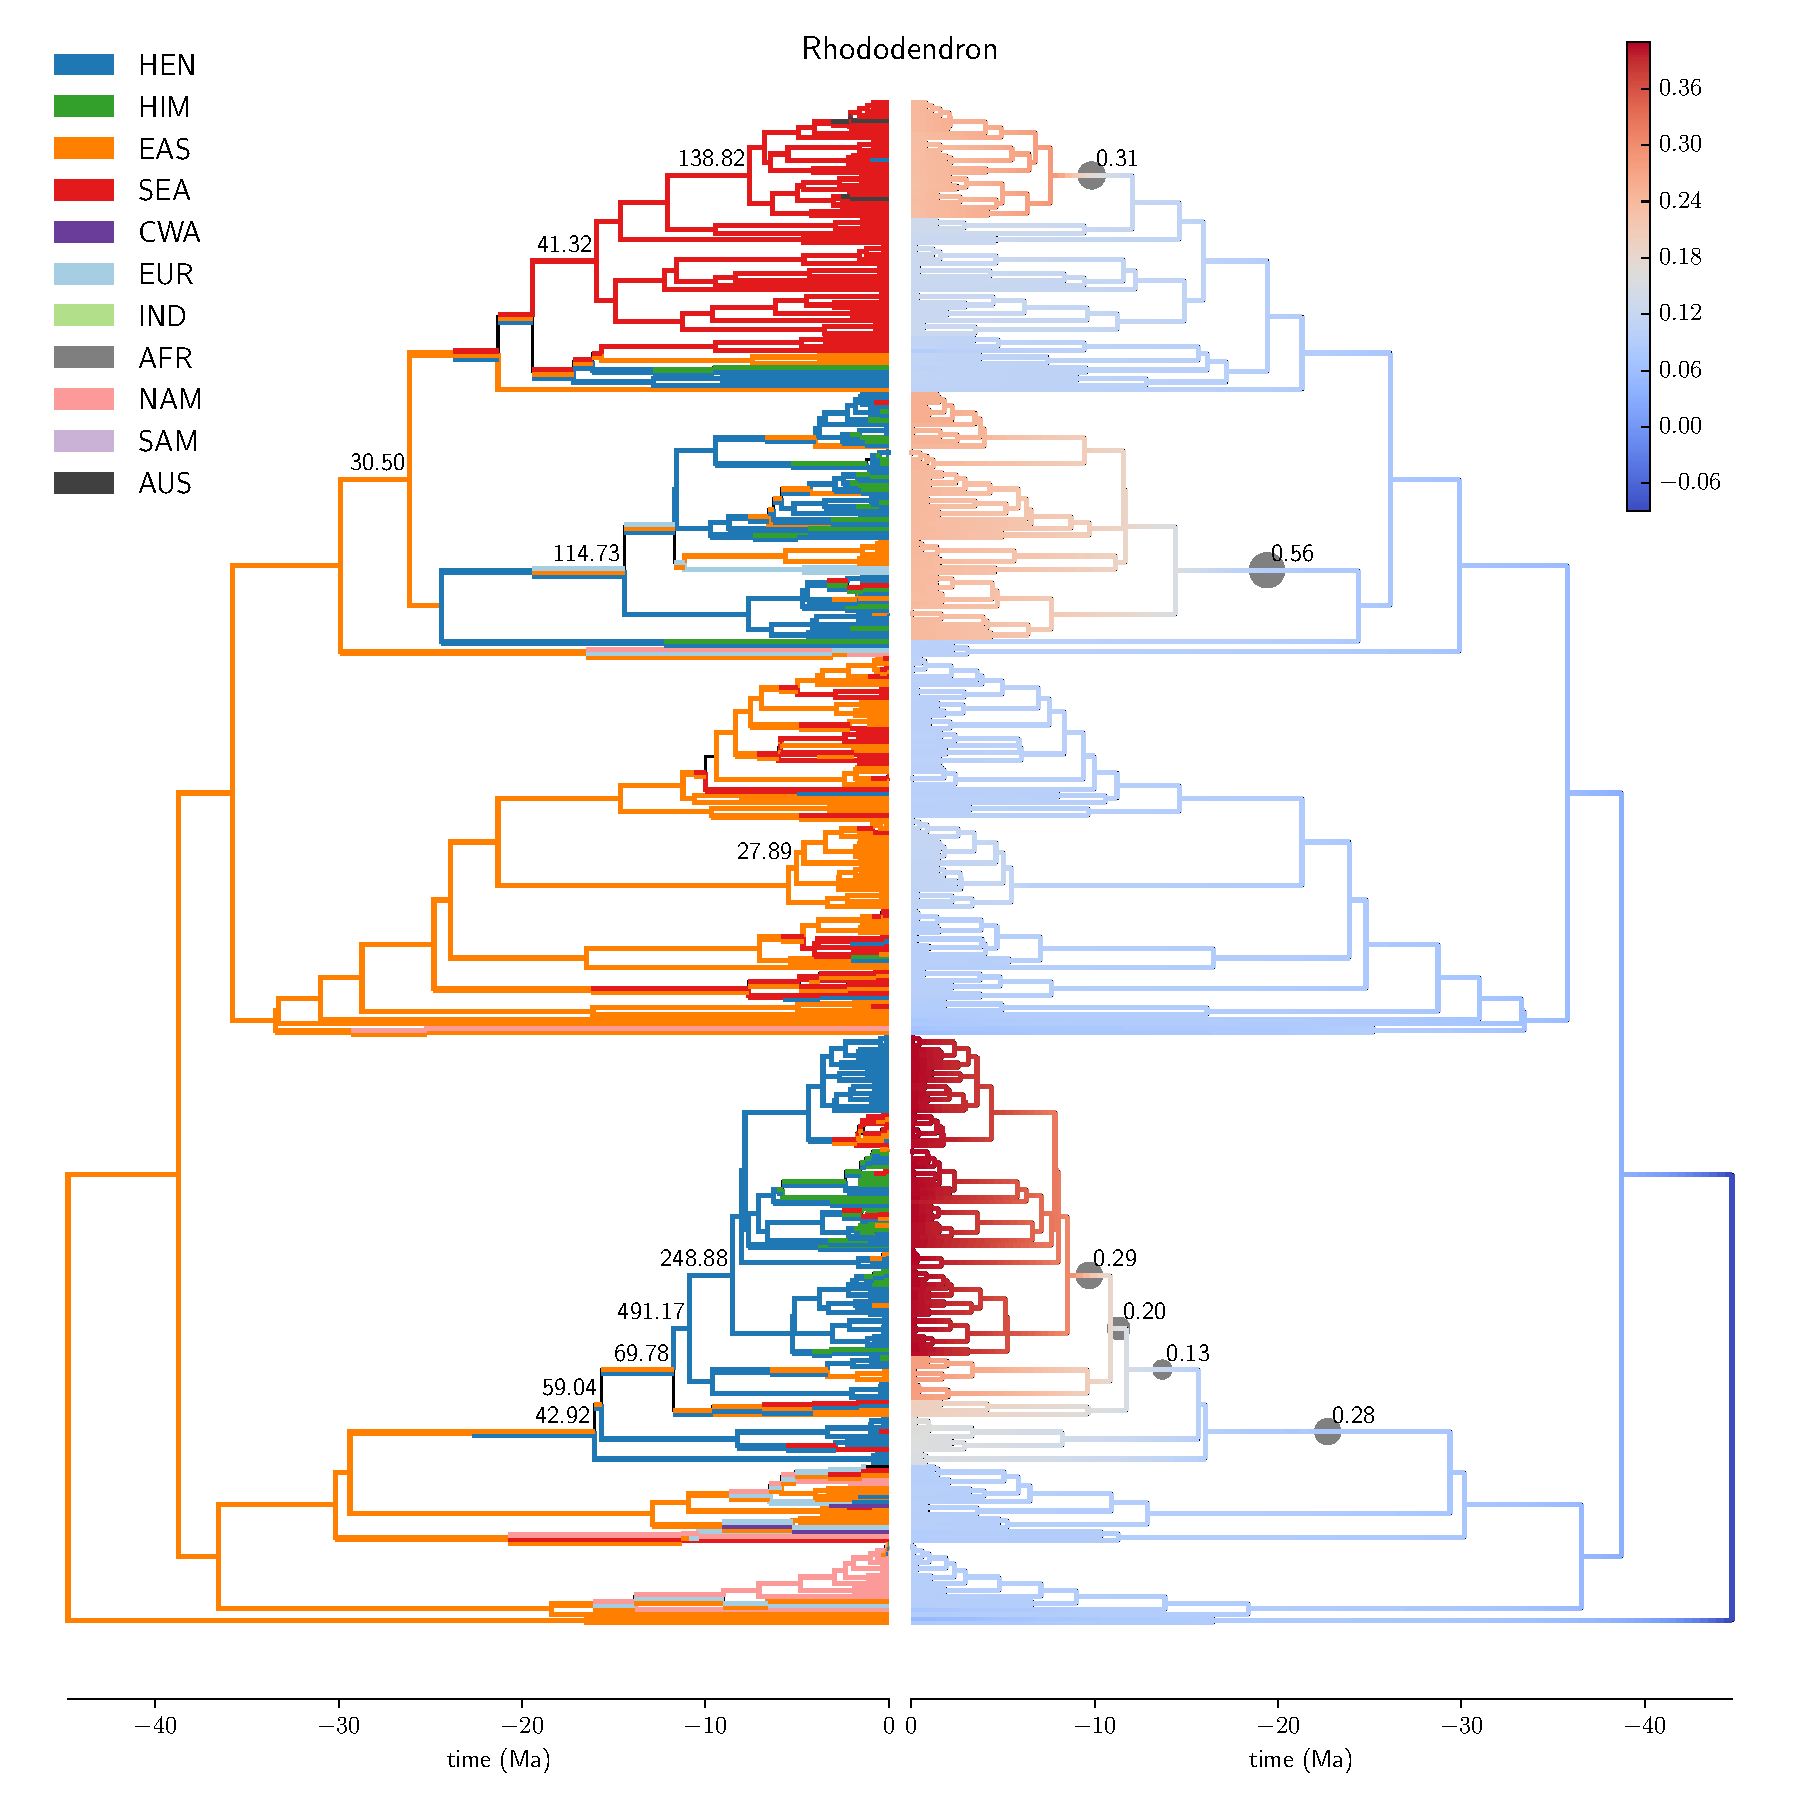
\includegraphics[width=.99\linewidth]{figures/Rhododendron-supfig/Rhododendron-supfig.pdf}
\caption{Reconstructions of ancestral geographic range (left) and net
  diversification rate (right) on the maximum clade credibility tree,
  with branch lengths set to posterior means, for
  \textit{Rhododendron}. Ancestral ranges are maximum-likelihood
  estimates at the start and end of each branch. Net diversification
  values are branch-segment means of the posterior distribution
  estimated by BAMM. Filled circles on the right indicate branches
  that appear in the 95\% credible set of distinct shift
  configurations, with the size and label of a circle indicating the
  cumulative probability of the branch over all configurations in the
  credible set. On the left, the marginal odds ratio for a shift in
  diversification regime along a branch is drawn for branches where
  the ratio exceeds 20. Geographic regions are coded as follows: HEN,
  Hengduan Mountains; HIM, Himalayas-QTP; EAS, temperate-boreal East
  Asia; SEA, Southeast Asia; CWA, central/western Asia; EUR, Europe;
  IND, India; AFR, Africa; NAM, North America; SAM, South America;
  AUS, Australasia. Hengduan species cluster primarily in 2 clades,
  both of which show evidence of ancestral shifts to higher
  diversification rate in the mid-to-late Miocene.}
\label{fig:rhododendron}
\end{figure}

\matmethods{
\section{Materials and Methods}

\subsection{Clade selection and phylogeny reconstruction}

Our criteria were that each clade (1) included a substantial number of species that occur in the Hengduan Mountains, as well as their closest known relatives in other biogeographic regions; (2) had sufficient molecular data available to infer a phylogeny that was broadly representative of the clade's taxonomic diversity and geographic range; and (3) had fossil data suitable for molecular clock calibration or secondary calibrations inferred from fossil dated phylogenies. We found 18 clades---16 of angiosperms and one each of gymnosperms (Pinaceae) and ferns (Microsorioideae)---that met these criteria. The combined taxon sample included a total of 3,262 ingroup species, of which 899 occur in the Hengduan Mountains region, 624 in the Himalayas-QTP, and 1,165 in the remainder of temperate/boreal East Asia (see \textit{Delimitation of biogeographic regions}). Of these, about 370 species are shared by the Hengduan Mountains and Himalayas-QTP regions. Across clades, the proportion of species sampled ranged from 20--97\% globally and 40--97\% for the Hengduan Mountains region (Table S1).

For each clade, we assembled molecular sequence alignments (Table S2; \textit{Appendix 1}) and fossil calibration data, and used relaxed molecular clock models implemented in BEAST 1.8 \citep{Drummond2012} or 2.0 \citep{Bouckaert2014} to generate a Bayesian posterior sample of time-calibrated phylogenies and the associated maximum-clade-credibility tree.  Detailed information is provided in \textit{SI Materials and Methods}.

%, representing approximately XX\%, YY\%, and ZZ\% of the vascular flora of each region (SI REF).

\subsection{Inference of range evolution and lineage diversification}

\subsubsection{Delimitation of biogeographic regions}

We defined 11 biogeographic regions (Fig.~S1), balancing considerations of model complexity, the need to accommodate the global distributions of the selected clades, and the granularity of our species range data. Of primary importance was distinguishing the Hengduan Mountains region from the geologically older parts of the QTP, especially the Himalayas. To that end, our definition of the Hengduan Mountains region follows \citet{Boufford2014}, and is bounded to the west by the Yarlung Tsangpo River in eastern Xizang (Tibet), to the northwest by the high plateau in Qinghai, to the north by the Tao River in southern Gansu, to the east by the Sichuan Basin, and to the south by subtropical forests and the Yunnan–Guizhou Plateau. As a primary point of comparison, we defined the ``Himalayas-QTP'' region as including the plateau itself, the Himalayas to the south, the Kunlun Mountains to the north, and the Qilian Mountains to the northeast. The other regions we defined are: temperate/boreal East Asia (the eastern boreal part of Russia and temperate regions of East Asia, including Japan and Taiwan); central/western Asia (including the Xinjiang Uyghur Autonomous Region to the south of Kunlun Range); southeast Asia (including tropical regions of China, Malesia, and Papuasia); Australasia (Australia, New Zealand, and the southwestern Pacific); India (south of the Himalyas, including Sri Lanka); Africa; Europe; North America; and South America (south of the Panama Canal). We scored the geographic range of each sampled species as its presence or absence in these regions based on floras, online databases, and published data sets (\textit{Dataset S1}; see also \textit{SI Materials and Methods}).

\subsubsection{Ancestral range reconstruction}

We set up a DEC model of range evolution in Lagrange \citep{Ree2005,Ree2008}, specifying a region-adjacency matrix that defined the valid set of spatially contiguous ranges. We explicitly avoided placing any temporal constraints on dispersal, so that biogeographic inferences were independent of prior beliefs about the ages of the Hengduan Mountains or Himalayas-QTP regions. For each clade, we used the model to infer a distribution of phylogenetic histories of biogeographic events. A single history for a clade was generated by sampling a chronogram from its Bayesian posterior distribution, estimating the maximum-likelihood set of ancestral ranges (geographic speciation scenarios) at internal nodes, and randomly interpolating parsimonious sequences of dispersal and local extinction events along branches having different ancestral and descendant ranges. This yielded a complete chronology of biogeographic events, i.e., where and when ancestral lineages moved and underwent speciation and local extinction. To account for phylogenetic uncertainty, one history was generated for each of 500 chronograms drawn randomly from the posterior for each clade. For further details, see \textit{SI Materials and Methods}.

\subsubsection{Regional assembly processes through time}

We focused our analysis on the dynamics of the Hengduan Mountains region in comparison to the Himalayas-QTP and temperate East Asia. Our objective was to estimate, for each region, rates of \textit{in situ} diversification and colonization and their cumulative contributions to biotic assembly through time. Taking the biogeographic histories of clades from the ancestral-range analysis, we generated 500 pseudoreplicated joint histories---sets of one history drawn randomly from each clade's pool without replacement. From each joint history, we extracted the chronology of \textit{in situ} speciation, colonization, and local extinction events affecting the 3 regions of interest and binned them into 1 Myr periods. This allowed region-specific estimates of assembly processes through time. We calculated rolling estimates of \textit{in situ} speciation rates as $\lambda(t) = s(t)/n(t-1)$, where $s(t)$ is the number of \textit{in situ} speciation events inferred in a region in a 1-Myr period $t$ and $n(t-1)$ is the number of inferred lineages in the region in the previous period (the cumulative sum of \textit{in situ} speciation and colonization minus local extinction). We also calculated rolling rates of colonization between regions as $d_{ij}(t) = c_{ij}(t)/n_i(t-1)$, where $c_{ij}(t)$ is the number of inferred colonization events of area $j$ from area $i$. For all estimates, confidence intervals (5--95\% quantiles) were calculated from the pseudoreplicated joint histories. Further details are provided in the \textit{SI Materials and Methods}.

\subsubsection{Geography-independent rates of diversification}

To complement the regional-process analysis and to better understand heterogeneity in rates of lineage diversification independently of geography, we generated Bayesian inferences of diversification rate for each clade using BAMM \cite{Rabosky2014}, which uses Markov chain Monte Carlo procedures to jointly estimate the number, parameters, and locations of distinct macroevolutionary regimes (rates of lineage birth and death, possibly time-dependent) on a phylogenetic tree. BAMM is able to account statistically for incomplete taxon sampling, so we assigned sampling fractions at the finest level of taxonomic resolution possible: this was generally at the level of genus, but at the level of section for \textit{Rhododendron} and \textit{Acer}. In cases where genera were not confidently resolved as monophyletic, we assigned sampling fractions at the higher taxonomic levels (tribe and subfamily). We ran each BAMM MCMC for 100 million generations with a sampling frequency of 1000 and assessed convergence by visually inspecting plots of the likelihood trace and calculating the effective sample size after discarding the first 10\% of the run as burn-in. We identified the 95\% credible set of distinct shift configurations and the overall best set of rate shifts given the data using the BAMMtools package in R \cite{Rabosky2014}.
}
\showmatmethods
%%% Local Variables:
%%% mode: latex
%%% TeX-master: "master"
%%% End:


\acknow{Y.X.\ was supported by the Boyd Postdoctoral Fellowship at the
  Field Museum and by a Swiss Advanced Postdoc.Mobility Fellowship
  (P300P3\_158528) and Pioneer Hundred Talents Program of the Chinese
  Academy of Sciences. The authors thank D.~Boufford for comments on a
  draft.}

\showacknow % Display the acknowledgments section


% \pnasbreak splits and balances the columns before the references.
% If you see unexpected formatting errors, try commenting out this line
% as it can run into problems with floats and footnotes on the final page.
\pnasbreak

\bibliography{bibliography/biblio}
%\bibliographystyle{ecol_let}
%\bibliographystyle{pnas2011}

\end{document}

%%% Local Variables:
%%% mode: latex
%%% TeX-master: t
%%% End:
